\chapter{Fundamentos Teóricos}
\label{cap:fundamento}
Este capítulo aborda conceitos e técnicas que fundamentam este trabalho. Será apresentado uma introdução sobre conceitos de redes neurais artificiais, bem como os fundamentos teóricos de aprendizado de máquina. Nas seções seguintes será abordado com mais detalhes o aprendizado por reforço, assim como a técnica de aprendizado utilizada neste trabalho. 

%% - - - - - - - - - - - - - - - - - - - - - - - - - - - - - - - - - - -
\section{Redes Neurais Artificiais}

Na busca de construção de máquinas inteligentes, um modelo a ser seguido é o do cérebro humano. As Redes Neurais Artificiais (RNA) são modelos computacionais inspirados pelo sistema nervoso central dos seres humanos, capazes de automatizar a aprendizagem por meio da análise de dados. As RNAs são compostas por nós interconectados onde cada nó, também conhecido como unidades lógicas, são os modelos matemáticos de neurônios artificiais \cite{gama11}. 

Na Figura \ref{fig:neuronio} é representado um modelo simples de neurônio artificial \cite{haylin99}. Cada neurônio recebe valores de entrada $x_{1}, x_{2}, ..., x_{n} $, que são ponderados dados os pesos $w_{k1}, w_{k2}, ..., w_{k1}$, e então combinados em uma soma, gerando um valor de saída $v_{k}$.  Por fim, uma função de ativação $\varphi(.)$ é utilizada para determinar como o valor gerado irá se propagar para outros neurônios. 

\begin{figure}[hb]
 \centering
  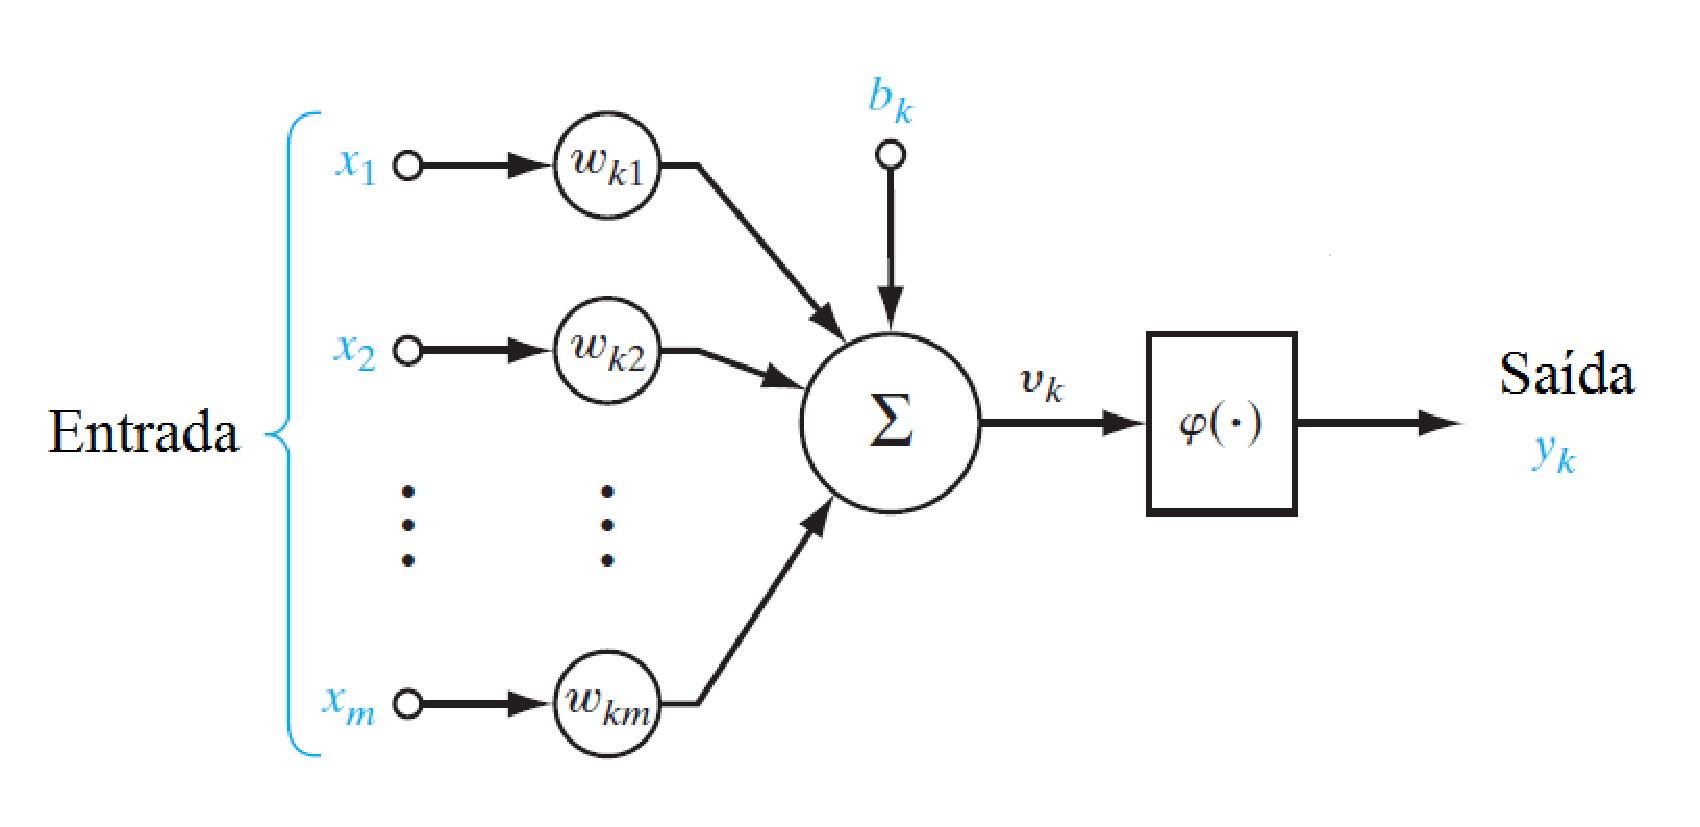
\includegraphics[width=0.7\textwidth]{./fig/neuronio}
 \caption{Modelo de um neurônio artificial \cite{santamaria2018}.}
 \label{fig:neuronio}
\end{figure}

Os pesos podem assumir valores positivos ou negativos, sendo seus valores ajustados em um processo de otimização, codificando o conhecimento adquirido pela rede. O modelo também inclui um \textit{bias} $b_{k}$, utilizado para aumentar o grau de liberdade dos ajustes dos pesos, permitindo uma melhor adaptação, por parte da rede neural, ao conhecimento a ela fornecido.

As funções de ativação introduzem um componente não linear às redes neurais, fazendo com que aprendam mais do que relações lineares entre as variáveis dependentes e independentes. Elas basicamente decidem se um neurônio deve ser ativado ou não, ou seja, se a informação que o neurônio está recebendo é relevante ou deve ser ignorada \cite{deeplearningb}.  Alguns exemplos de funções de ativação são observados na Figura \ref{fig:activacao}.

\begin{figure}[ht]
  \centering
  \subfigure[Degrau]
   {
    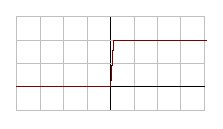
\includegraphics[width=0.3\textwidth]{./fig/Activation_binary_step}
    \label{subfig:bi}
   } 
  \subfigure[Sigmoidal]
   {
    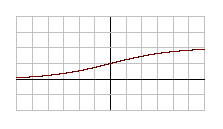
\includegraphics[width=0.3\textwidth]{./fig/Activation_logistic}
    \label{subfig:sig}
   }
   \subfigure[Gaussiana]
   {
    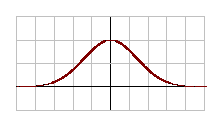
\includegraphics[width=0.3\textwidth]{./fig/Activation_gaussian}
    \label{subfig:gauss}
   }
   \caption{Exemplos de funções de ativação.}
  \label{fig:activacao}
\end{figure}

Os neurônios costumam ser divididos em camadas, onde existe uma camada de neurônios de entrada, podendo ser conectada a uma ou diversas camadas intermediárias que, por sua vez, se conectam aos neurônios da camada de saída, como mostra a Figura \ref{fig:redeneural}. A camada de entrada é responsável pelo recebimento dos dados a serem analisados, assim como a correspondente associação com os pesos de entrada. As camadas intermediárias tem por finalidade extrair as informações associadas ao sistema inferido, sendo também responsável pela maior parte do processamento destes dados. Já a camada de saída agrega as informações das camadas anteriores e ativa uma resposta adequada.

\begin{figure}[H]
 \centering
  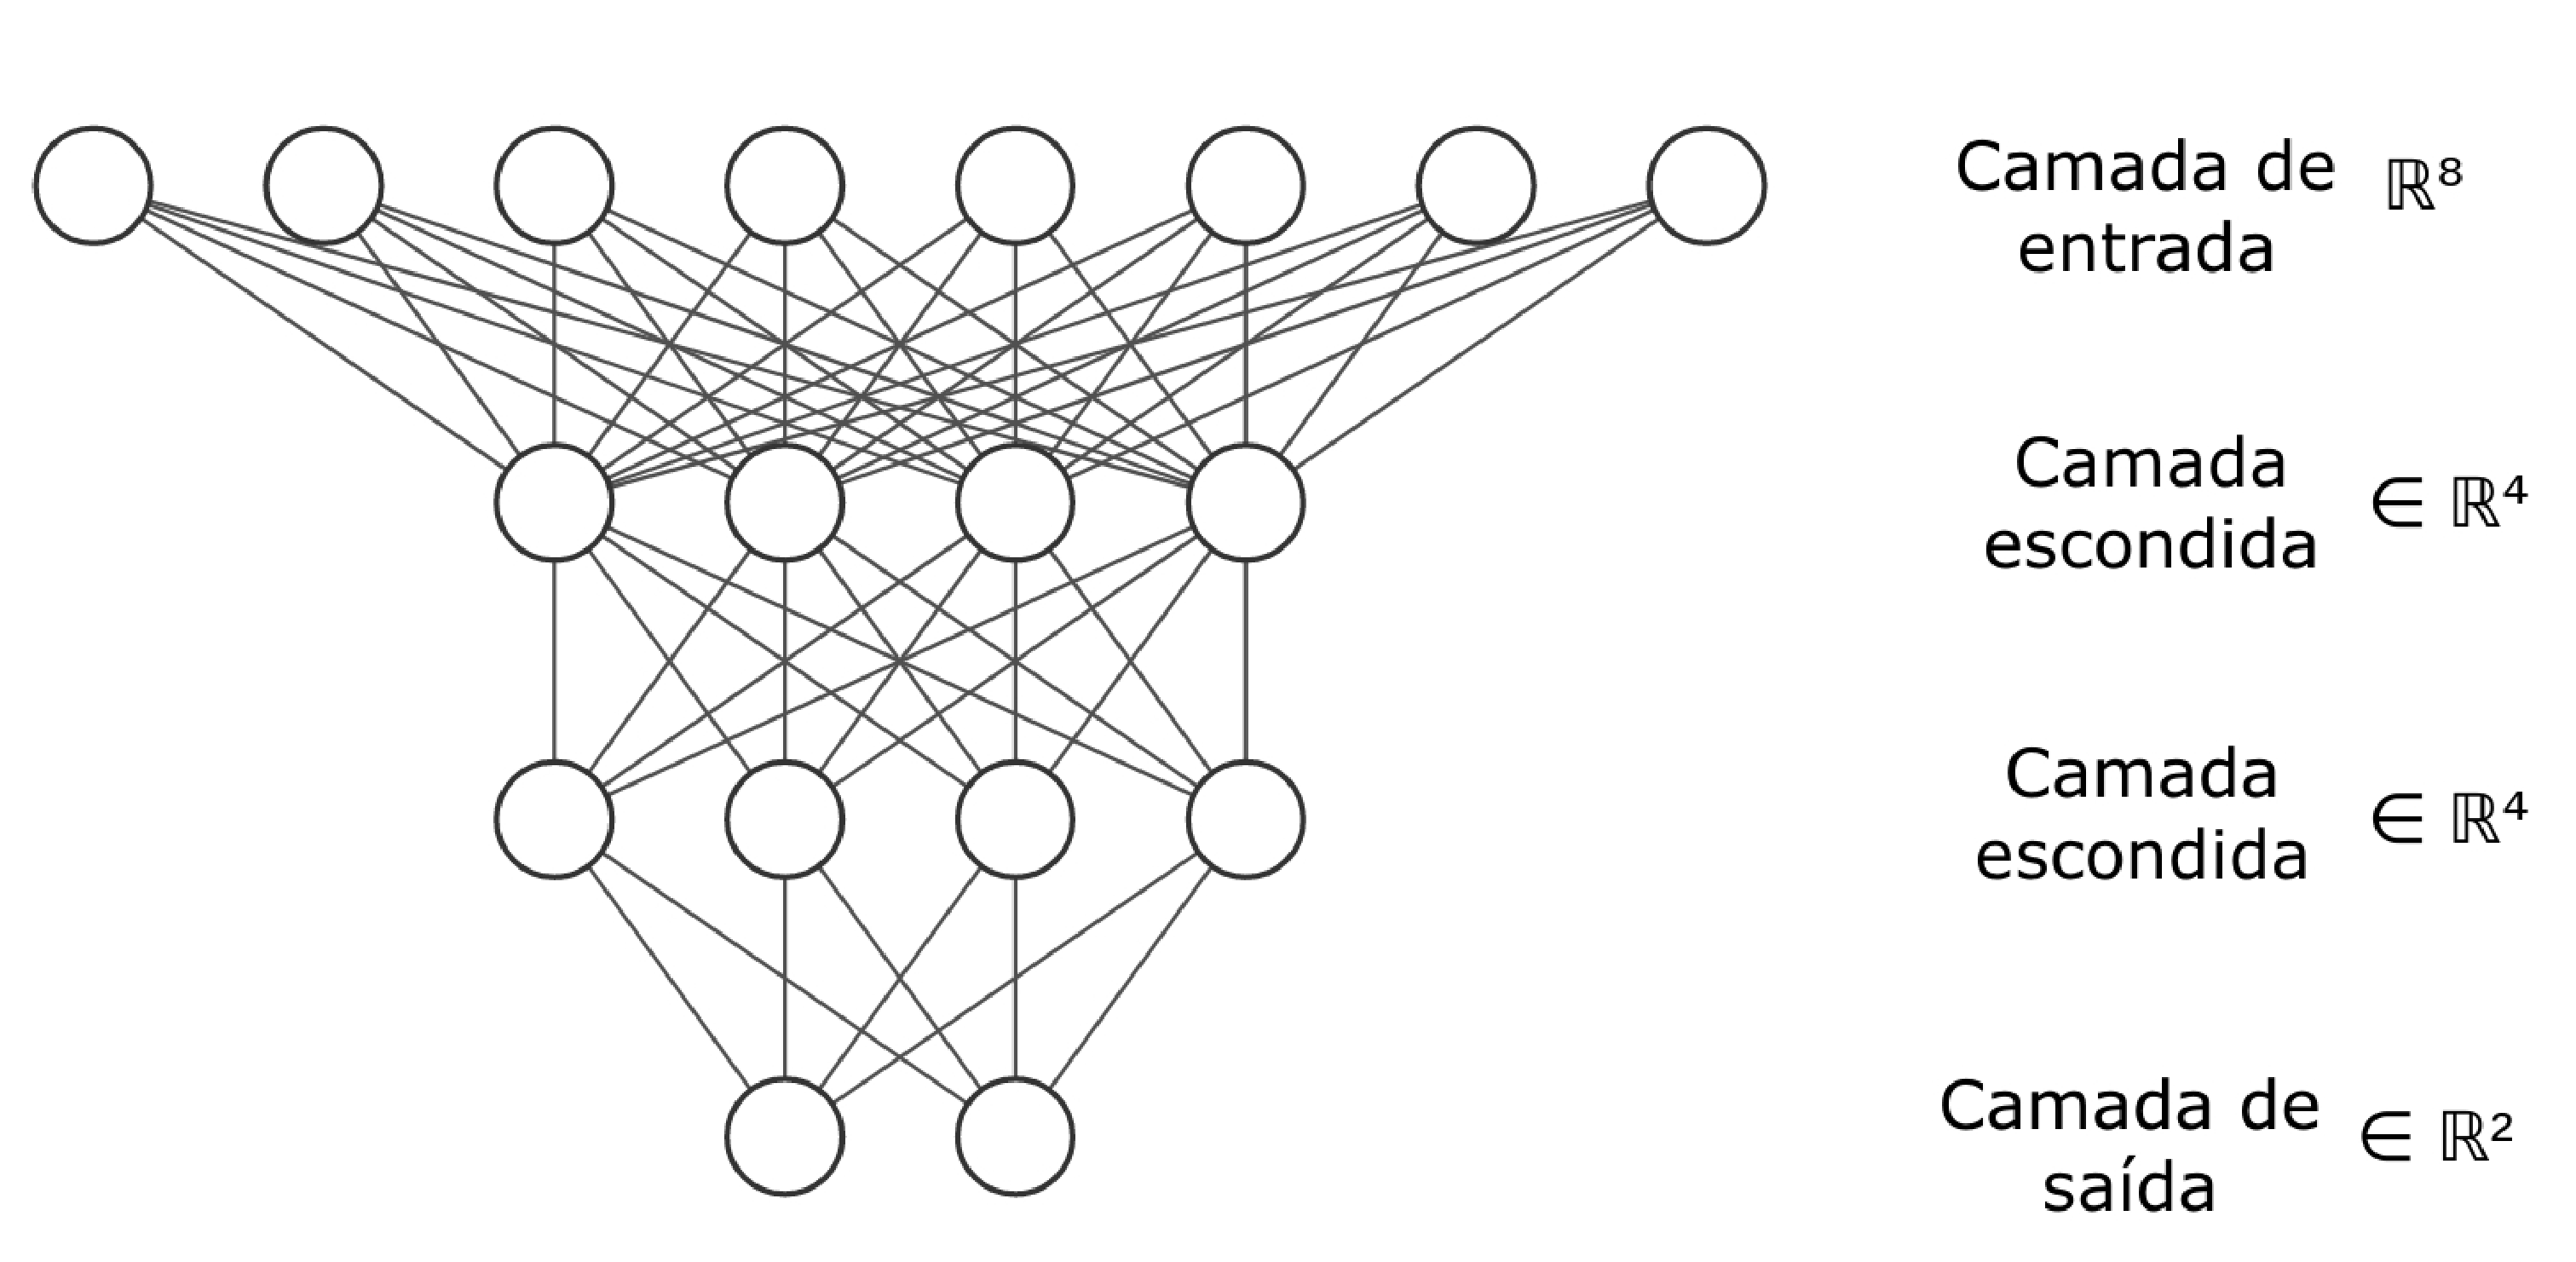
\includegraphics[width=0.8\textwidth]{./fig/nn}
 \caption{Rede neural com duas camadas intermediárias.}
 \label{fig:redeneural}
\end{figure}

Redes neurais com muitas camadas intermediárias são ditas redes neurais profundas. Nessas redes, os dados são submetidos a um processo de várias etapas de reconhecimento de padrões, cada camada sendo é responsável por reconhecer um conjunto de características diferente. Quanto mais profundo na rede, mais complexas serão as características reconhecidas, uma vez os dados são agregados e recombinados da camada anterior. 

As conexões de uma RNA define como os neurônios são conectados entre si, podendo ser classificadas em redes diretas (\textit{feedforward}) ou redes recorrentes. Nas redes diretas, as informações fluem da camada de entrada para os neurônios da camada de saída. Já as conexões das redes recorrentes permitem que um neurônio receba a saída de um neurônio da mesma camada, de uma camada posterior, ou até mesmo a sua própria saída. Os sistemas baseados em RNAs, dependem fortemente da topologia destas redes (tamanho, estrutura, conexões), assim como de seus parâmetros. Como resultado, a determinação da arquitetura da rede afeta muito o seu desempenho, isto é, velocidade de aprendizado, exatidão do aprendizado, tolerância a ruídos e capacidade de generalização.

Dentre as topologias existentes, têm-se as Redes Neurais Convolucionais (CNN, do inglês \textit{Convolutional Neural Network}), que utilizam uma arquitetura especial que é particularmente bem adaptada para classificar imagens \cite{Krizhevsky12}. O ponto central de uma CNN são as camadas convolucionais, que dão o nome da rede. Uma convolução, nesse contexto, é uma operação linear que envolve a multiplicação de um conjunto de pesos ao conjunto de entrada. Como a entrada dessa rede é de natureza bi-dimensional, a multiplicação é realizada entre a entrada e vetores bi-dimensionais de pesos, chamados de filtros. Cada um dos filtros é responsável por aprender uma determinada característica nos dados de entrada.

Um método comum para o treinamento de uma rede neural é o algoritmo de \textit{backpropagation}  \cite{rumelhart86}. Em um processo de otimização, a rede neural transmite o sinal dos dados de entrada até a camada de saída, através de seus parâmetros. O gradiente de uma função de custo é então retro-propagado pela rede para que seus pesos possam ser alterados, visando minimizar essa função. 

Nas últimas décadas, com a crescente complexidade dos problemas a serem tratados computacionalmente e do volume de dados gerados por diferentes setores, o uso de RNA se tornou cada vez mais comum. As redes neurais profundas são responsáveis por avanços recentes em uma grande variedade de tarefas difíceis de se resolver utilizando programação baseada em regras comuns, como, por exemplo, áreas de visão computacional \cite{Krizhevsky12}, de reconhecimento de fala \cite{NassifSAAS19} e do processamento de linguagem natural \cite{otter2018}.

%% - - - - - - - - - - - - - - - - - - - - - - - - - - - - - - - - - - -
\section{Aprendizado de Máquina}

% Um algoritmo é uma sequência de ações/etapas que levam à uma solução de um problema. Na computação, portanto, um algoritmo é uma ferramenta para solucionar problemas computacionais descritos e especificados, dado um conjunto de entrada. Entretanto, alguns problemas são difíceis de se estabelecer uma sequência de passos finitos para ser realizado, ou obter uma sequência de passos que irão gerar um conjunto de saída em um tempo não exorbitante. Um mundo onde tem-se uma carga de informação impossível de ser acompanhada por qualquer ser humano, onde há toneladas de dados e informações a serem analisadas, a Inteligência Artificial (IA) entra como agente capaz de automatizar a aprendizagem repetitiva por meio da análise de dados.

O aprendizado de máquina pode ser definido como a área da Inteligência Artificial relacionada à busca de um conjunto de regras/padrões que permitem que as máquinas tomem decisões baseadas em um grande conjunto de dados sem serem especificamente programadas para essa tomada de decisões \cite{Samuel59}. Em outras palavras, o aprendizado de máquina é o processo de encontrar um modelo ou hipótese que aproxima uma função alvo usando um conjunto de dados de treinamento. Depois que a máquina é treinada, a hipótese final deve satisfazer os dados de treinamento bem como dados não vistos anteriormente.

Tradicionalmente, essa área é dividida em três diferentes categorias, baseadas na natureza do tipo de aprendizagem: aprendizado supervisionado, aprendizado não supervisionado, e aprendizado por reforço. Além disso, há abordagens de otimização estocástica, como computação evolutiva, para aprendizado \cite{Salimans2017}. Todas essas abordagens são candidatas viáveis de treinamento para jogos eletrônicos \cite{justesen2018}.

O Aprendizado Supervisionado consiste na tarefa de inferir uma função a partir de dados de treinamento rotulados (par composto por um objeto de entrada e um valor de saída desejado), com a finalidade de prever rótulos desconhecidos em um conjunto de teste, podendo o rótulo ser um conjunto finito ou um valor real. Em contra-partida, no aprendizado não supervisionado não há nenhum tipo de orientação para verificar se a predição está correta e o objetivo passa a ser encontrar padrões nos dados. Já no aprendizado por reforço, um agente interage com um ambiente e seu o objetivo é aprender um comportamento através dessa interação, visando maximizar um valor de retorno, chamado de recompensa.

%% - - - - - - - - - - - - - - - - - - - - - - - - - - - - - - - - - - -
\section{Aprendizado por Reforço}

Aprendizado por reforço é a área de aprendizado de máquina cujo objetivo reside em criar agentes artificiais que possuem a capacidade de alcançar um nível equivalente de performance e generalização dos seres humanos \cite{deepmind}. 

O aprendizado se dá pela interação do agente com o ambiente em que ele se encontra. Essa interação é representada pela escolha de ações a serem executadas no ambiente, que levam a mudanças de estados. Dessa interação, o agente obtém sinais de retorno, que irão categorizar se a ação tomada foi uma boa ou má escolha. Os sinais de retorno, também chamados de recompensa, podem ocorrer com frequência, como a alteração na pontuação dentro de um jogo, ou com pouca frequência, como se um agente ganhou ou perdeu um jogo. Todo esse processo de escolhas de ações se dá por tentativa e erro do agente, tornando esse modelo de aprendizado o mais próximo do processo de aprendizado dos seres humanos e animais.

Um Processo de Decisão de Markov (MDP, do inglês \textit{Markov Decision Process}) fornece uma estrutura matemática para modelagem de tomada de decisão em situações onde os resultados são em parte aleatórios e em parte sob o controle de um tomador de decisão \cite{sutton-barto98}. Se um ambiente pode ser descrito como um MDP, então o agente pode construir uma árvore de probabilidade de estados futuros e suas recompensas, que poderá ser utilizada para calcular o valor do estado atual \cite{Lapan2018}. A figura \ref{fig:rl} mostra a interação agente-ambiente em um MDP.

\begin{figure}[ht]
 \centering
  \includegraphics[width=0.70\textwidth]{./fig/RL}
 \caption{Interação agente-ambiente em um Processo de Decisão de Markov \cite{sutton-barto98}.}
 \label{fig:rl}
\end{figure}

Temos que um MDP consiste de um conjunto finito de estados $S$, um conjunto de possíveis ações $A(s)$ para cada estado, um valor de retorno $R$ para cada estado, e um modelo de transição $P(s'|s,a)$. Para cada episódio no tempo $t$, o retorno é definida por:

\begin{equation}
R_t = r_{t+1} + \gamma r_{t+2} + ... =  \sum^{\infty}_{k=0}\gamma^k r_{t+k+1}
\end{equation}

O retorno é calculado como uma soma de recompensas subsequentes. Um fator de desconto $\gamma$ é utilizado para recompensas mais distantes do ponto de início $t$, definindo a visibilidade do agente. Entretanto, esse valor de retorno a longo prazo não é muito útil na prática: o agente pode tomar diferentes ações resultando em diferentes caminhos para um mesmo estado \cite{Lapan2018}. Para isso, temos uma função de retorno mais útil, a função de valor (Equação \ref{eqn:value}), que consiste na predição do valor de retorno a longo prazo.

\begin{equation}
\label{eqn:value}
V(s) = \E \left[\sum^{T}_{t=1}\gamma^{t-1}r_{i}\right] \forall s \in S
\end{equation}

A função de valor representa o quão bom um estado é com base em sua recompensa. O objetivo do agente é maximizar esse valor. Entretanto, para alcançar bons estados é necessário escolher ações que levam para esses estados. Para isso, temos a política, que define o comportamento do agente, ou seja, uma política diz para o agente o que fazer em uma determinada situação \cite{Lapan2018}. Formalmente, política é definida como uma distribuição de probabilidades sobre ações $a$ para cada possível estado $s$ em um dado tempo $t$ (Equação \ref{eqn:estocastico}), ou como um simples mapeamento de estados para ações (Equação \ref{eqn:determistico}).

\begin{equation}
\label{eqn:estocastico}
\pi(a|s) = P(A_t = a|S_t = s)
\end{equation}

\begin{equation}
\label{eqn:determistico}
\pi(s) = a
\end{equation}

Há algumas abordagens para resolver um problema de aprendizado por reforço. Dentre elas temos os métodos baseados em valor e métodos baseados em política. Métodos baseados em valor focam em encontrar ou aproximar a função de valor ideal que maximizam a recompensa, enquanto sua política é mantida de tal forma a escolher o par de ação-estado que obtém a maior recompensa. Métodos baseados em política, tentam encontrar a política ideal diretamente, sem consultar a função valor, buscando também maximizar a recompensa. Ambos os métodos baseados em valor e em política são ditos livre de modelo, ou seja, ignoramos o modelo e dependemos apenas da amostragem e simulação para estimar as recompensas, para que não seja preciso conhecer o funcionamento interno do sistema. Já métodos baseados em modelo, se podemos definir uma função de recompensa, podemos calcular as ações ideais usando o modelo diretamente. 

Mesmo não precisando levar em consideração a política durante o aprendizado, todo algoritmo de aprendizado por reforço deve seguir alguma política para decidir quais ações executar em cada estado. Algoritmos que levam em consideração a política que gerou decisões passadas de ação-estado são chamados de algoritmos \textit{on-policy}, enquanto aqueles que a ignoram são conhecidos \textit{off-policy}. Algoritmos \textit{off-policy} geralmente empregam uma política de comportamento separada, independente da política que está sendo aprimorada; a política de comportamento é usada para simular trajetórias. Um algoritmo \textit{off-policy} bem conhecido é o \textit{Q-Learning} \cite{Watkins92}. Sua regra de atualização usa a ação que produzirá o \textit{Q-Value} mais alto, enquanto que a verdadeira política usada pode restringir essa ação ou escolher outra. O \textit{Q-value} é uma medida da recompensa geral esperada, assumindo que o agente esteja no estado $s$ e executa uma ação $a$, e continua a jogar até o final do episódio, seguindo alguma política $\pi$. A variação \textit{on-policy} do \textit{Q-learning} é o SARSA \cite{rummery94}, onde a regra de atualização usa a ação escolhida pela política seguida.


%% - - - - - - - - - - - - - - - - - - - - - - - - - - - - - - - - - - -
\section{Métodos de Gradiente de Política}

Em métodos baseados em política e, em especial, métodos de gradiente de política, o objetivo é aprender uma política que consegue selecionar ações sem consultar a função de valor diretamente. Nesse método a política pode ser tanto determinística quanto estocástica, além de ser possível de se trabalhar com um espaço de ações contínua \cite{Lapan2018}. Quando o agente obtém uma observação e precisa tomar uma ação precisamos da política, ou seja, é da política que precisamos ao resolver um problema de aprendizado de reforço.

Como qualquer configuração de aprendizado de máquina, pode-se definir um conjunto de parâmetros $\theta$ (como por exemplo, os pesos e \textit{bias} das redes neurais) para parametrizar uma política - $\pi_{\theta}$. O objetivo é buscar os parâmetros $\theta$ que maximizam a recompensa obtida, portanto, uma abordagem para resolver esse problema é o método do gradiente (Equação \ref{eqn:objpg}). No gradiente, continuamente percorremos os parâmetros usando a regra de atualização da Equação \ref{eqn:pgrad}. A recompensa $R_t$ guia a atualização, enquanto que a taxa de aprendizado $\alpha$ define a magnitude do ajuste feito nas atualizações \cite{sutton-barto98}.

\begin{equation}
\label{eqn:objpg}
\nabla_{\theta}J(\theta) = \E_{t\sim\pi_{\theta}} \left[\sum^{T}_{t=0}\nabla_{\theta}log\pi_{\theta}(a_t|s_t)R_t\right]
\end{equation}

\begin{equation}
\label{eqn:pgrad}
\theta_{t+1} = \theta_{t} + \alpha \nabla_{\theta} J(\pi_{\theta_k})
\end{equation}

A Equação \ref{eqn:objpg} mede a probabilidade da trajetória sob a política atual. O uso da função de recompensa aumenta a probabilidade de uma política se a trajetória resultar em uma alta recompensa positiva. Por outro lado, diminui a probabilidade de uma política se resultar em uma alta recompensa negativa. Entretanto, a função de recompensa pode impedir a exploração de políticas que poderiam levar a uma recompensa maior, uma vez que um único caminho que leva o agente obter recompensas positivas seria reforçado sempre. O método de gradiente é um método de derivada de primeira ordem, não sendo muito confiável se a função de recompensa tiver uma curvatura muito íngreme \cite{jonathanHuiRL}. Para resolver isso, é utilizado a função de vantagem (Equação \ref{eqn:advantage}) em vez da recompensa esperada, por reduzir a variação da estimativa \cite{jonathanHuiPPO}.

\begin{equation}
\label{eqn:advantage}
A_{t}^{(n)}(s,a) = r_{t} + \gamma V(s_{t+1}) + ... + \gamma^n V(s_{t+n}) - V(s_{t})
\end{equation}

A função de vantagem é uma medida de quanto uma determinada ação é uma decisão boa ou ruim, dado um determinado estado. Em outras palavras, a função informa sobre a recompensa extra que poderia ser obtida pelo agente, executando essa ação específica. Se $A_{t}(s,a) > 0$ o gradiente é empurrado nessa direção. Se $A_{t}(s,a) < 0$, ou seja, a ação escolhida é pior que o valor médio desse estado, o gradiente é empurrado na direção oposta.

A Equação \ref{eqn:advantage} assume a forma de estimadores de diferença temporal, onde primeiro é estimado a soma das recompensas com desconto e então é descontado a estimativa da função de valor. Para $A_{t}^{(n)}$ com valores baixos de $n$ a estimativa terá baixa variação, mas alto viés, enquanto para valores altos de $n$ a estimativa terá viés baixo, mas alta variação \cite{seita}. Dado esse dilema de viés e variância, foi proposto uma abordagem mais geral para calcular a vantagem, a Estimativa de Vantagem Generalizada (GAE, do inglês \textit{Generalized Advantage Estimation}) \cite{Schulman16}.

\begin{equation}
\label{eqn:temporaldiscount}
\delta^{V}_{t} = r_{t} + \gamma V(s_{t+1}) - V(s_{t})
\end{equation}

\begin{equation}
\label{eqn:gae}
A_{t}^{GAE(\gamma, \lambda)} = \sum_{l=0}^{\infty} \left(\gamma\lambda\right)^{l}\delta^{V}_{t}
\end{equation}

A Equação \ref{eqn:gae} é um estimador de vantagem com dois parâmetros separados $\gamma$ e $\lambda$, os quais contribuem para o balanceamento entre a variação e o viés. No entanto, ambos os parâmetros servem a propósitos diferentes e funcionam melhor com diferentes faixas de valores \cite{Schulman16}. O fator $\gamma$ ainda definirá o desconto de recompensas futuras, enquanto que o fator $\lambda$ é responsável pelo balanceamento entre o viés e a variação.


%% - - - - - - - - - - - - - - - - - - - - - - - - - - - - - - - - - - -
\section{\textit{Proximal Policy Optimization}}
\label{section:ppoalg}

Alguns problemas dos métodos de gradiente de política aparecem da taxa de aprendizado: se for muito pequena o processo de treinamento será muito lento, porém se for muito alta terá muita variabilidade no treinamento. A ideia central do algoritmo \textit{Proximal Policy Optimization} (PPO) \cite{Schulman17} é evitar grandes atualizações de políticas. A taxa de aprendizado restringe as atualizações relacionadas aos parâmetros, enquanto que o PPO leva em consideração as probabilidades das ações, utilizando uma proporção que indica a diferença entre uma nova política e uma política antiga (Equação \ref{eqn:ratio}). Como as probabilidades das ações que definem o comportamento da política, estabilizá-los entre as atualizações garante uma maior estabilidade \cite{Schulman15}. 

\begin{equation}
\label{eqn:ratio}
r_{t} = \frac{\pi_{\theta}(a_{t}|s_{t})} {\pi_{\theta_{old}}(a_{t}|s_{t})} 
\end{equation}

Se $r_{t}(\theta) > 1$ então a ação é mais provável na política atual do que na política antiga, enquanto que se $r_{t}(\theta)$ está entre 0 e 1 a ação é menos provável na nova política do que na antiga. Entretanto, a ausência de uma restrição pode levar a grandes atualizações \cite{Schulman17}. O que o PPO faz é tentar garantir pequenas alterações restringindo a razão de probabilidade das políticas, penalizando grandes passos que levam a políticas muito diferentes. Dessa maneira teremos duas proporções, uma sem restrição e uma restringida a um intervalo (entre $[1-\epsilon, 1+\epsilon]$, onde $\epsilon$ é um hiper-parâmetro). Então, pega-se o mínimo entre esses valores, sendo o objetivo final um limite inferior para a atualização da política, evitando grandes atualizações. A nova função objetivo fica definida como:

\begin{equation}
\label{eqn:clip}
L^{CLIP}(\theta) = \E_{t} \left[min(r_{t}(\theta)A_{ t}, clip(r_{t}(\theta), 1-\epsilon, 1+\epsilon)A_{t}\right]
\end{equation}

\begin{figure}[ht]
 \centering
  \includegraphics[width=0.80\textwidth]{./fig/clip}
  \captionsetup{width=1\textwidth}
 \caption[Gráficos da função $L^{CLIP}$.]
 {Gráficos da função $L^{CLIP}$. Valores em função da razão de probabilidade $r$, para vantagens positivas (esquerda) e vantagens negativas (direita) \cite{Schulman17}.}
 \label{fig:ppoclip}
\end{figure}

A nova função objetivo (Equação \ref{eqn:clip}) reduz a vantagem estimada se a nova política estiver longe da antiga. Se uma ação é muito mais provável sob a nova política do que a antiga, não queremos exagerar na atualização da ação, então restringimos a função objetivo. Se a nova política for muito menos provável do que a antiga, novamente deve-se impedir atualizações exageradas.

O PPO tenta delimitar uma pequena região para atualizações, mas trata o problema como um método iterativo de otimização, onde é possível utilizar gradiente ascendente. O Algoritmo \ref{alg:ppoclip} representa o funcionamento do PPO com objetivo limitado \cite{Achiam}. Primeiro, avalia-se a política sobre um conjunto de dados, e então realiza-se melhorias aplicando atualizações de otimização da Equação \ref{eqn:clip}. Durante o período de avaliação, a função de vantagem $A^\pi$ da política atual $\pi$ será estimada. Em seguida, é possível modificar a política atual executando atualizações com base na função de vantagem. Depois de gerar essa nova política, voltamos à avaliação. Esse ciclo ocorre até encontrarmos a função de vantagem e política ideais.


\medskip
\begin{center}
\begin{minipage}{0.92\textwidth}
\begin{algorithm2e}[H]
 \DontPrintSemicolon
 \Entrada{parâmetros da política inicial $\theta_0$, limiar de corte $\epsilon$}
 \Para{$k= 0, 1, 2, ...$}
   {Colete um conjunto de trajetórias $D_k$ com política $\pi_k = \pi(\theta_{k})$ \\
    Estime a função de vantagem $A_{t}^{GAE(\gamma, \lambda)}$ \\
    Calcule a atualização da política \\
    \hspace{3cm}$\theta_{k+1} = arg \max_{\theta}L^{CLIP}_{\theta_k}(\theta)$ \\
    executando N etapas do gradiente ascendente, onde \\
    \hspace{2cm}$L^{CLIP}_{\theta_k}(\theta) = \E_{t} \left[min(r_{t}(\theta)A_{ t}, clip(r_{t}(\theta), 1-\epsilon, 1+\epsilon)A_{t}\right]$ 
   }
\caption{\textit{Proximal Policy Optimization} com objetivo limitado \label{alg:ppoclip}}
\end{algorithm2e}
\end{minipage}
\end{center}
